\chapter{Initial Condition Response from Vertical Position}\label{app:fallResponseAppendix} 
\textbf{Name: Group 630}\\
\textbf{Date: 17/03 - 2016}

\subsubsection{Purpose}
Find the fall response of the frame from the vertical position, \si{\theta_F=0}, and from a \si{10^\circ} tilted position.
Data is used to compare the measured response and the simulation given by the theoretical nonlinear model.

\subsubsection{Setup}
The wheel is being held in a fixed position with a strip tied to it and the frame. The probe chosen is a 1:1 and is connected to the potentiometer with probe to yellow cable and ground clamp to brown cable. The power supply has to be turned on in order to get readouts from the potentiometer. A sponge is placed on the rubber pad in order to damp the impact of the frame.
\begin{figure}[H]                                   
	\centering                                        
	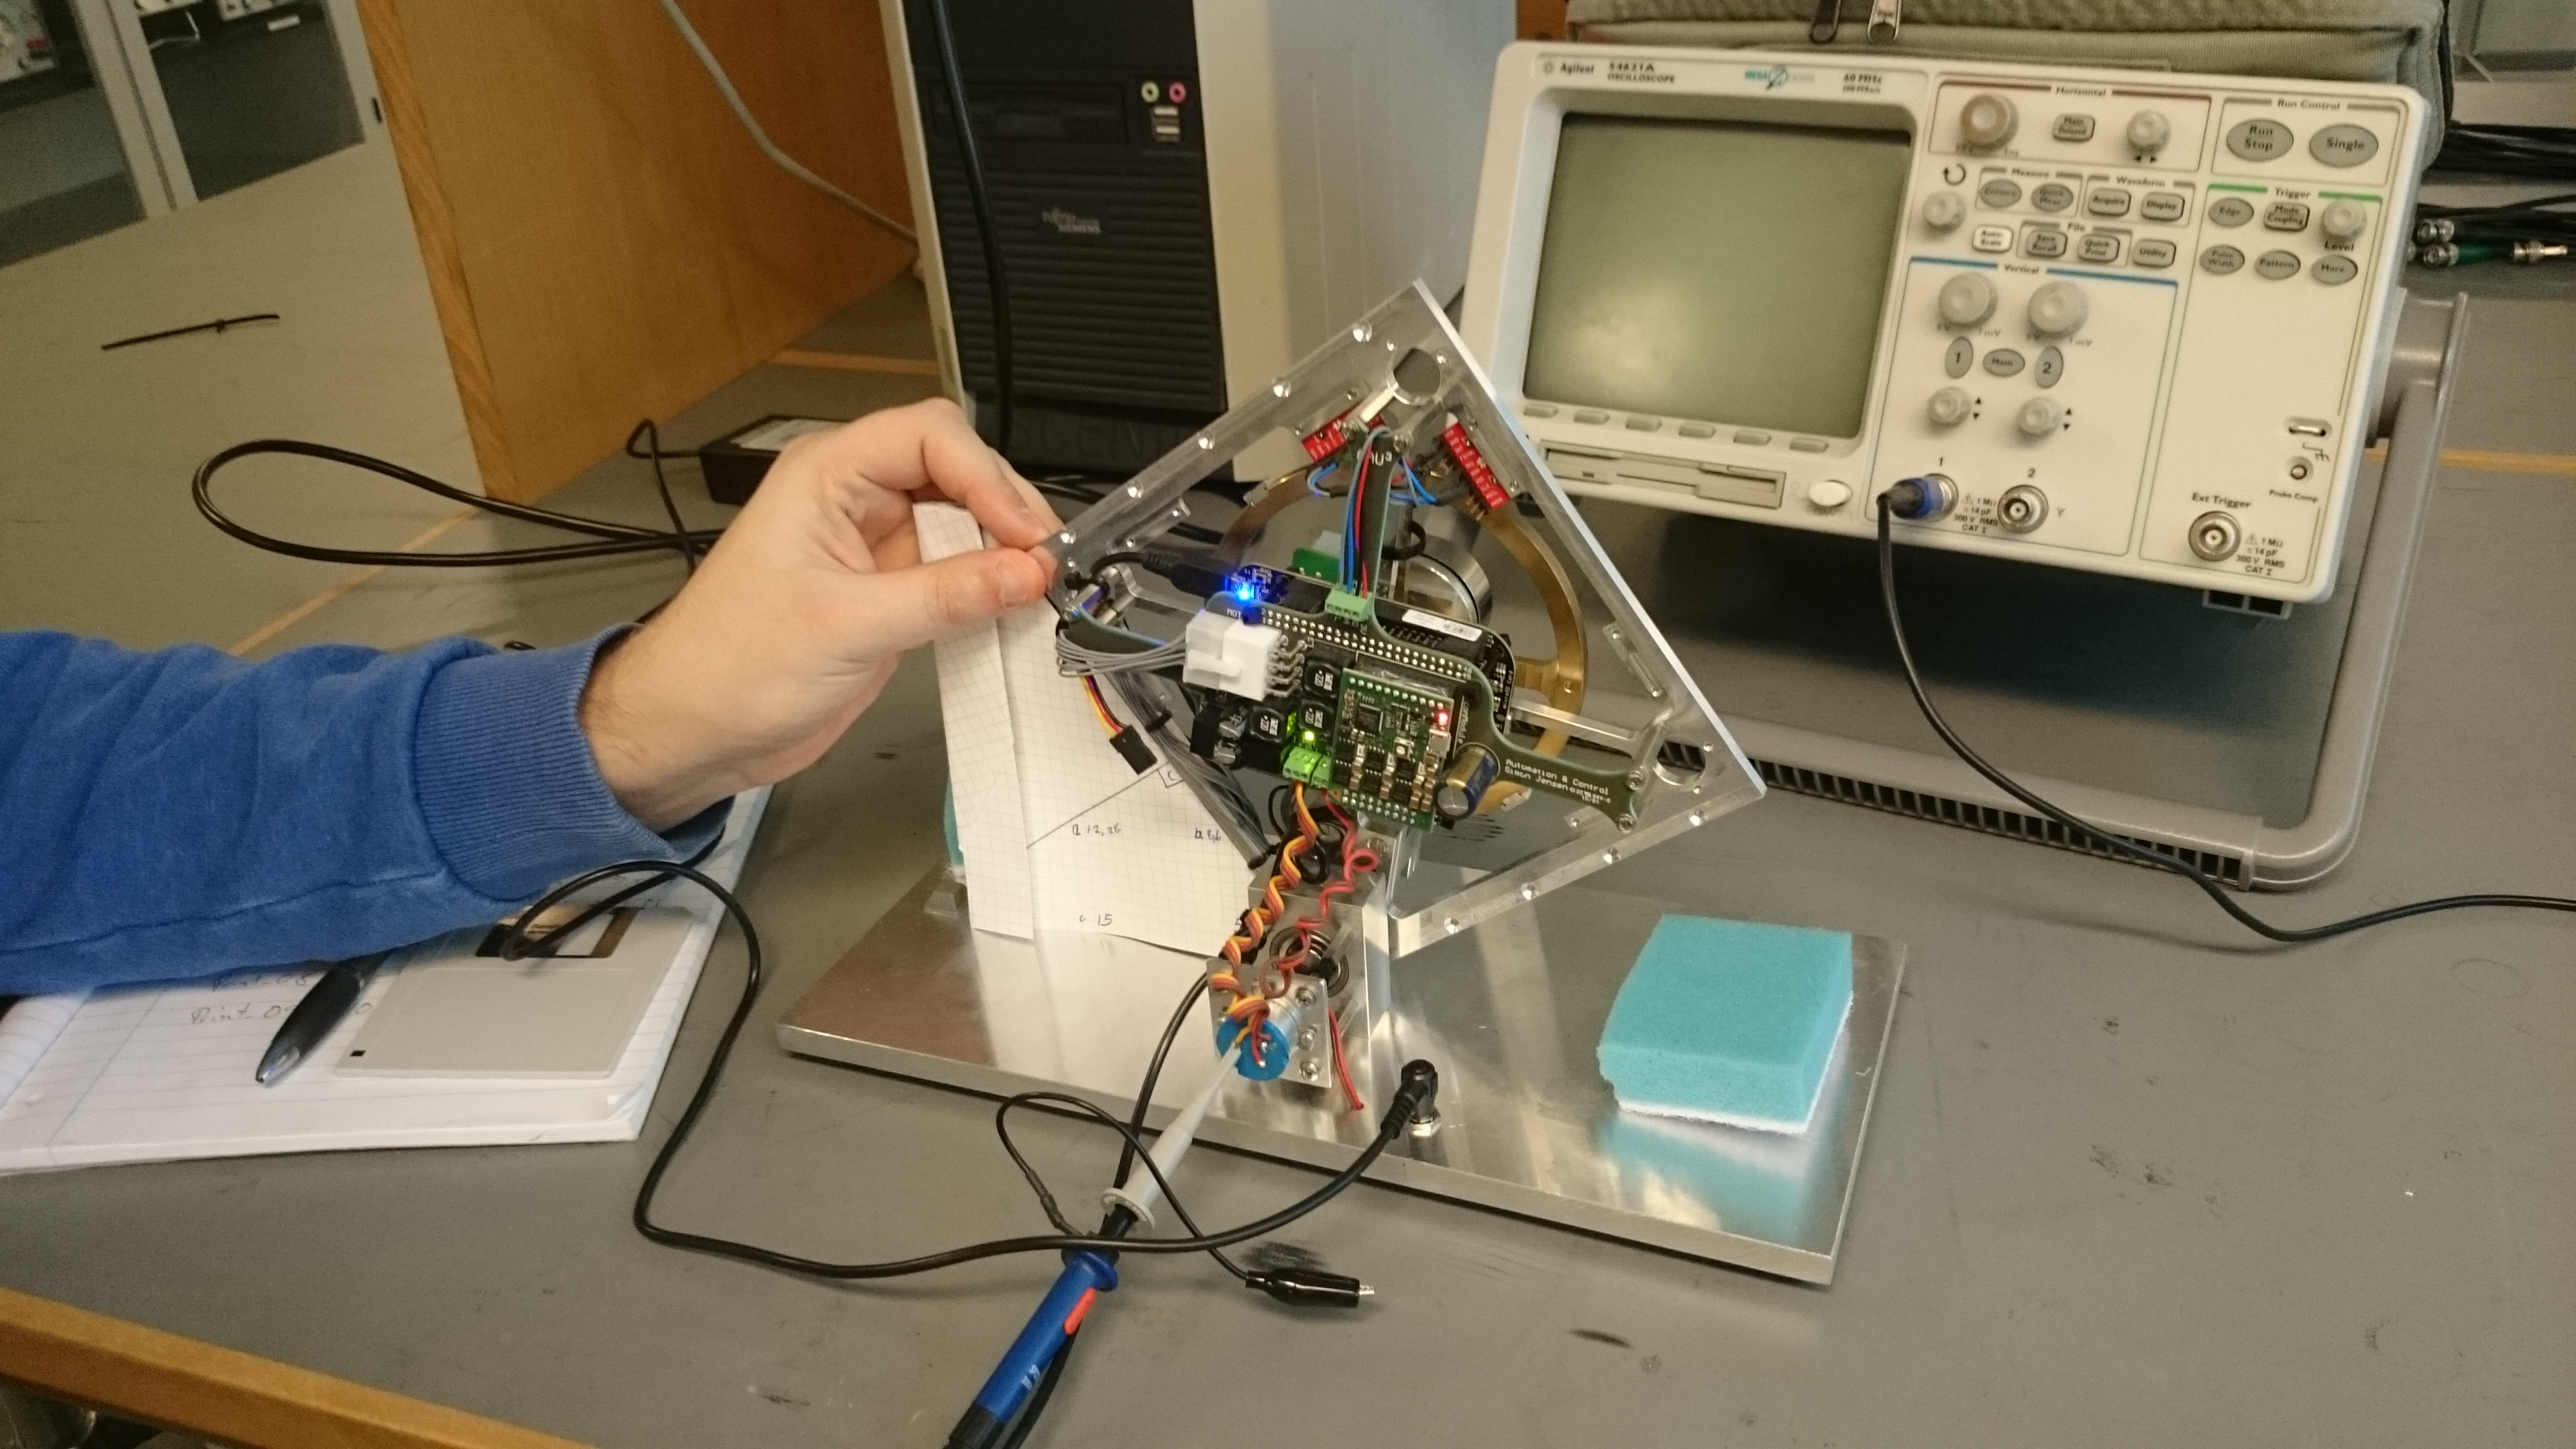
\includegraphics[scale=0.08]{figures/stepResponseSetup}
	\caption{Picture of the setup for the fall-response test}
	\label{stepResponseTestPicture} 
\end{figure}              

\subsubsection{List of Equipment}
\begin{table}[H]
	\begin{tabular}{|l|l|p{4.3cm}|}
		\hline%------------------------------------------------------------------------------------
		\textbf{Instrument}                        &  \textbf{AAU-no.}  &  \textbf{Type}       \\
		\hline%------------------------------------------------------------------------------------
		Cubli setup                              &               &  		  \\
		\hline%------------------------------------------------------------------------------------
		Oscilloscope                              &  61604             &  Agilent 54621A		  \\
		\hline%------------------------------------------------------------------------------------
		Dedicated Power Supply of Cubli \small{(24 V - 3 A)} &               &  XP Power, AEB70US24 \\
		\hline%------------------------------------------------------------------------------------
		Probe 1:1                &  TBD            &          TBD   \\
		\hline%------------------------------------------------------------------------------------
		Sponge               & 5P0N63             &              \\
		\hline%------------------------------------------------------------------------------------
	\end{tabular}
\end{table}
fix of table\fxnote{find the probe used} 
\subsubsection{Procedure}
\begin{enumerate}
	%\item Turn on the power supply
	\item Keep the Cubli in the starting position (\si{0^\circ} or \si{10^\circ})
	\item Let the Cubli fall over
	\item Use the oscilloscope to measure the voltage changes in the potentiometer and save them
	\item Take the measurements and plot them in Matlab
	%\item Plot the result of the simulations in the same figure and compare them
\end{enumerate}

\subsubsection{Results}
Data from the test is presented in a graph showing the measured  voltage.
%The data is available as a .csv file on the CD
\fxnote{Make sure this is put into the CD folder for copying}

\small\textbf{Fall response starting from \si{0^\circ}}

\begin{minipage}{\linewidth}
	\begin{minipage}{0.45\linewidth}
		\begin{figure}[H]
			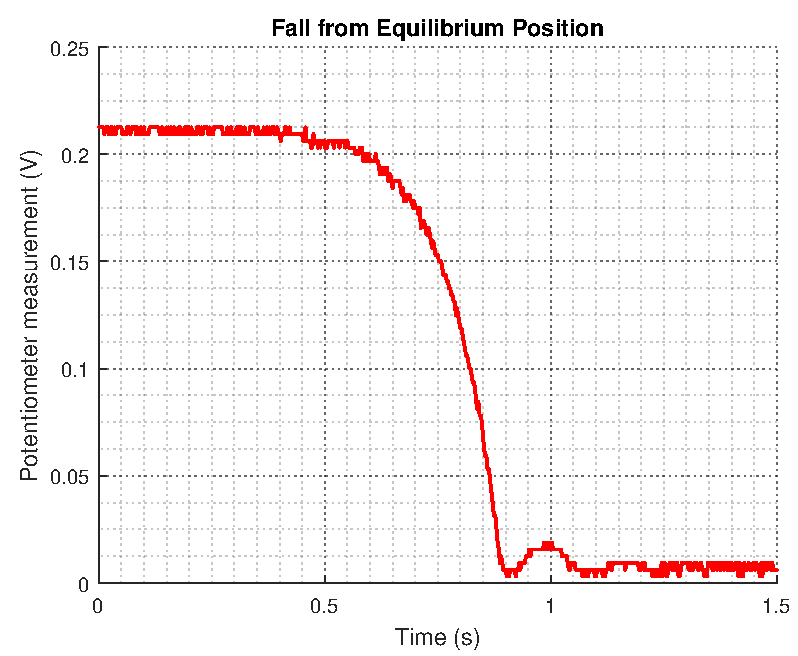
\includegraphics[scale=.53]{figures/FallVolt}
			\centering
			\vspace{-.4cm}
			\captionsetup{justification=centering}
			\captionof{figure}{Raw data taken from the potentiometer}
			\label{FallVolt}
		\end{figure}\vspace{-5mm}
	\end{minipage}
	\hspace{0.03\linewidth}
	\begin{minipage}{0.45\linewidth}
		\begin{figure}[H]
			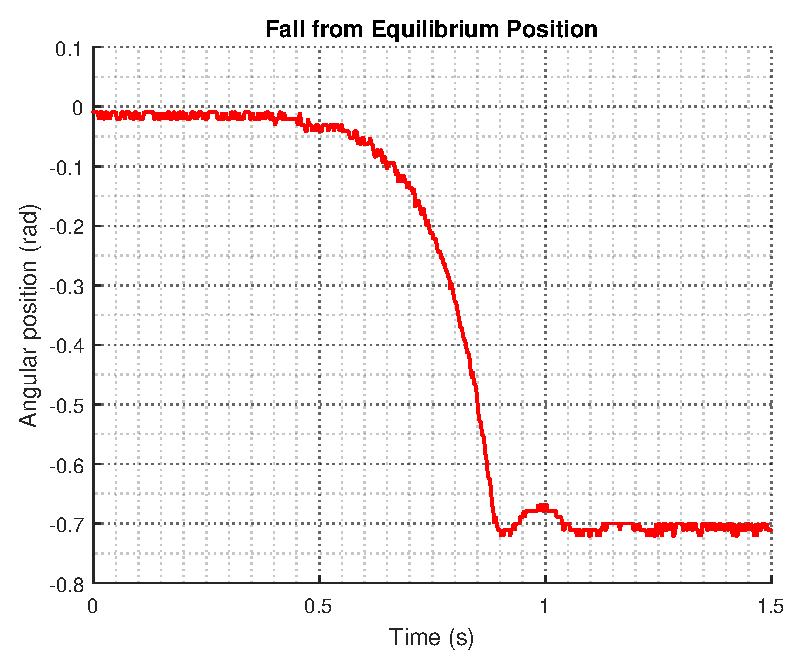
\includegraphics[scale=.53]{figures/FallRad}
			\centering
			\vspace{-.4cm}
			\captionsetup{justification=centering}
			\captionof{figure}{Angular position of the frame}
			\label{FallRad}
		\end{figure}\vspace{-5mm}
	\end{minipage}
\end{minipage} 

\small\textbf{Fall response starting from \si{10^\circ}}

\begin{minipage}{\linewidth}
	\begin{minipage}{0.45\linewidth}
		\begin{figure}[H]
			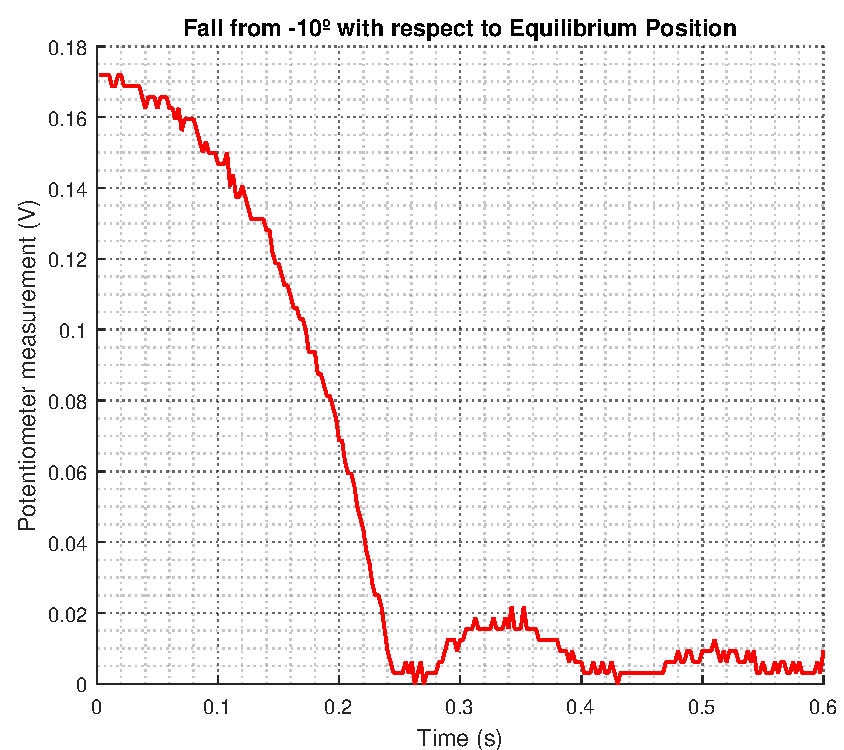
\includegraphics[scale=.53]{figures/tenDegFallVolt}
			\captionsetup{justification=centering}
			\captionof{figure}{Raw data taken from the potentiometer}
			\label{tenDegFallVolt}
		\end{figure}%\vspace{-5mm}
	\end{minipage}
	\hspace{0.03\linewidth}
	\begin{minipage}{0.45\linewidth}
		\begin{figure}[H]

			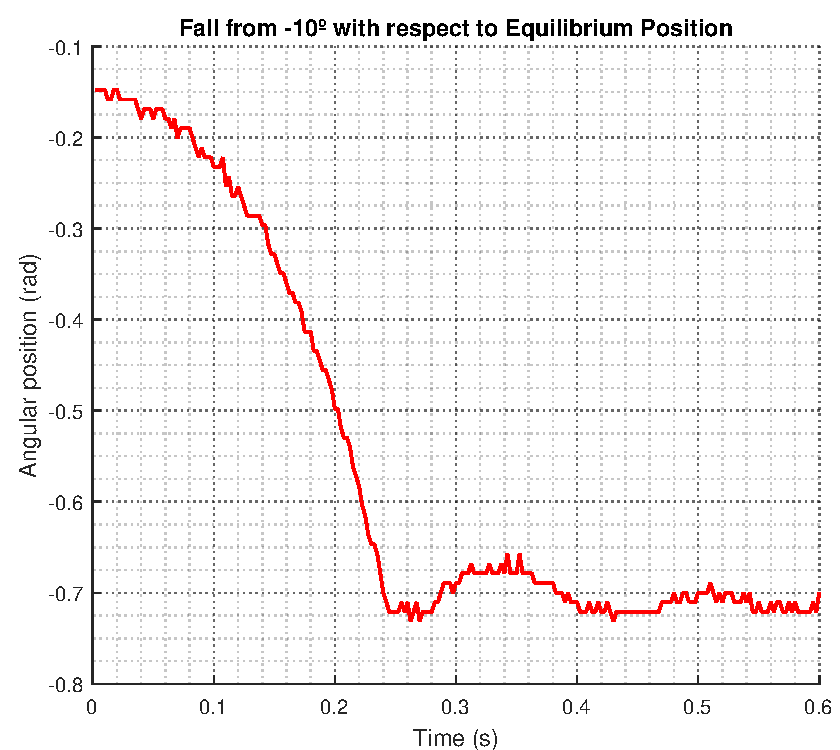
\includegraphics[scale=.53]{figures/tenDegFallRad}
			\captionsetup{justification=centering}
			\captionof{figure}{Angular position of the frame}
			\label{tenDegFallRad}
		\end{figure}%\vspace{-5mm}
	\end{minipage}
\end{minipage} \fxnote{Look at the layout of picture of data placement}


%The result of the experiment (\figref{comparisonRealModel}) shows that the response of the real system has several differences with the one from the simulation.
%
%The fist one is the presence of oscillations in the real response curve. This behavior is due to a small bounce that the frame does when it reaches the base.
%
%Another one is the final position of the frame, but it is due to the existence of a piece of foam at this position in the real case (to avoid the Cubli to hit the base).
%
%The other main difference is the shape of the curve, since the simulation is slower than the real case.

\subsubsection{Note}
The bouncing in the data when the frame reaches the lower position due to the presence of the sponge.




